\documentclass[11pt]{exam}
\usepackage{amsfonts,amsthm,amsmath,amssymb,mathrsfs,bbm,dsfont}
\usepackage{hyperref}
\usepackage{nicematrix}
\usepackage{csquotes}\MakeOuterQuote{"}
\qformat{\textbf{Problem \thequestion}\quad (\thepoints)\hfill}
\newcommand{\ind}{\perp\!\!\!\!\perp} 
\newtheorem{theorem}{Theorem}

\usepackage[backend=biber,style=nature]{biblatex}
%\bibliographystyle{unsrt}
\addbibresource{refs.bib}


\begin{document}

\begin{center}

     \textbf{Bi/BE/CS 183 2022-2023\\ Instructor: Lior Pachter\\ TAs: Tara Chari, Meichen Fang, Zitong (Jerry) Wang \vskip 0.15in Problem Set 4}

\end{center}
Submit your solutions as a single PDF file via Canvas by {\bf 8am Tuesday February 7th}. 
\begin{itemize}
  \item If writing up problems by hand, please use a pen and not a pencil, as it is difficult to read scanned submission of pencil work. Typed solutions are preferred.
  \item For problems that require coding, Colab notebooks will be provided. Please copy and save the shared notebook and edit your own copy, which you should then submit by including a clickable link in your submitted homework. Prior to submission make sure that you code runs from beginning to end without any error reports.
  \end{itemize}


\begin{questions}
\question[40] Given observed data $X$, unobserved/latent variable $Z$ and model parameter $\theta$, the Expectation-maximization (EM) algorithm attempts to maximize the following Q-function
\begin{equation}
\begin{split}
	Q(\theta\mid \theta_t) &= E_{Z|X,\theta_t}[\log p(X, Z;\theta)] \\
	&= \int p(Z|X;\theta_t) \log p(X,Z; \theta).
	\end{split}
\end{equation}
We will show that improving $Q(\theta | \theta_t)$ will indirectly improve the log-likelihood $\log p(X|\theta)$, and that $\log p(X|\theta)$ is guaranteed to be non-decreasing with each step of the algorithm.

\begin{parts} 
\part[10] Show that the log-likelihood of the observed data $\log p(X;\theta)$ can be expressed in term of the Q-function,
\[ \log p(X|\theta) = Q(\theta | \theta_t) - R(\theta | \theta_t),\]
where $R(\theta | \theta_t) = E_{Z|X,\theta_t}[\log p(Z | X; \theta)]$
\part[10] Show that for any $\theta$, the following inequality holds,
\[R(\theta | \theta_t) \leq R(\theta_t | \theta_t)\]
Hint: use the fact about the logarithm of a positive number x: $log(x) \leq x-1$ with equality if and only if x = 1.

\part[10] Denoting the estimated parameter at two consecutive step of the EM algorithm as $\theta_t$ and $\theta_{t+1}$, show that $\log p(X|\theta_{t+1}) - \log p(X|\theta_{t}) \geq Q(\theta_{t+1}| \theta_t) - Q(\theta_t | \theta_t)$. This shows that by improving the Q-function, the EM algorithm causes $\log p(X;\theta)$ to improve by at least as much.
\part[10] Show that for any step $t$ of the EM algorithm, the following holds
\[\log p(X|\theta_{t+1}) \geq \log p(X|\theta_{t}).\]
In other words, the log-likelihood is non-decreasing with every step of the EM algorithm.

\end{parts}
\newpage

\question[30] The EM procedure is often used to estimate relative abundances of transcripts as sequencing reads may align to multiple transcript sequences. To resolve these ambiguities the EM algorithm can be applied as shown below (Fig. 1). Given $N$ reads and $K$ transcripts, the reads are aligned to the transcript sequences to determine which transcript(s) they originate from. We can summarize this alignment with a matrix $\mathbf{Y}$ defined by $y_{k,n} = 1$ if read $n$ aligns to transcript $k$ and 0 otherwise. $\mathbf{Y}$ is denoted as the \textit{compatibility matrix}. For Fig. 1, with 5 reads and 3 transcripts, the compatibility matrix is 
\begin{figure}[!hb]
        \centering
        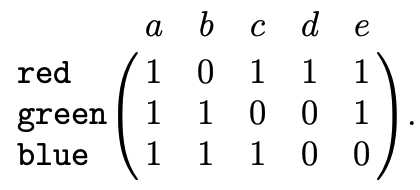
\includegraphics[scale=0.25]{Figures/compat.png}
    \end{figure}

For example $y[red,b] = 0$ as read $b$ (denoted by a black bar in Fig. 1) does not overlap with any part of transcript $red$ (read bars in Fig. 1). From these reads and their overlapping alignments, we want to estimate the relative abundances, denoted as $\alpha$, for each transcript, $(\alpha_1,...\alpha_k)$.

\begin{figure}[!hb]
        \centering
        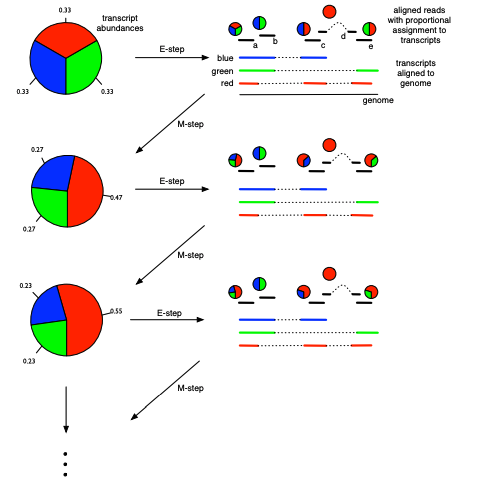
\includegraphics[scale=0.55]{Figures/emFig.png}
        \caption{Example of EM algorithm steps for 3 transcripts and 5 reads. From \cite{Pachter2011-tv}.}
    \end{figure}
    
For Fig. 1 , we are attempting to estimate the parameters $\alpha_{red}, \alpha_{green}, \alpha_{red}$, and given $\mathbf{Y}$ the likelihood to maximize is then \\
\begin{align*}
 \mathcal{L}(\alpha) &= \prod_{n=1}^{N} (\sum_{k=1}^{K} y_{k,n}\alpha_k) \\
  &=  (\alpha_{red} + \alpha_{blue})(\alpha_{red} + \alpha_{green})(\alpha_{blue} + \alpha_{green})\alpha_{red},
\end{align*}
subject to $ \alpha_{red} + \alpha_{blue} + \alpha_{green} = 1. $ \\

In the EM algorithm, we iteratively approximate the read counts given some $\alpha$ estimate (Fig. 1, E step), then we recalculate the $\alpha$ parameters given the (proportional) read counts (Fig. 1, M step). Denote the $\alpha$ in step t by $\alpha^{(t)}$. We will let the latent variable $Z$ denote whether a read comes from transcript $k$. \\

In the E-step, we first calculate the posterior distribution:
\begin{align}
    p(Z_n=k|Y_n;\alpha^{(t)})&= \frac{p(Z_n=k,Y_n|\alpha^{(t)})}{\sum_k p(Z_n=k,Y_n|\alpha^{(t)}) } \nonumber\\
    &= \frac{  y_{k,n} \alpha^{(t)}_{k}}{ \sum_{k=1}^K y_{k,n} \alpha^{(t)}_{k}}
\end{align}
Then the Q-function is 
\begin{align*}
    Q &= E_{Z|Y,\alpha^{(t)}}[\log p(Y, Z;\theta)] \\
    &=\sum_{n=1}^N E_{Z_n|Y_n,\alpha^{(t)}}[\log p(Y_n, Z_n;\alpha)] \\
    &=\sum_{n=1}^N \sum_{k=1}^K p(Z_n=k|Y_n;\alpha^{(t)}) \log p(Z_n=k, Y_n;\alpha) \\
    &=\sum_{n=1}^N \sum_{k=1}^K \frac{ y_{k,n} \alpha^{(t)}_{k} }{ \sum_{l=1}^K  y_{ln} \alpha^{(t)}_{l}} \log ( y_{k,n} \alpha_{k})
\end{align*}

In the M-step, $\alpha$ is optimized. Using a Lagrange multiplier and maximizing the following quantity
$$
\sum_{n=1}^N \sum_{k=1}^K \frac{  y_{k,n} \alpha^{(t)}_{k} }{ \sum_{l=1}^K  y_{l,n} \alpha^{(t)}_{l}} \log (y_{k,n} \alpha_{k}) - \lambda (\sum_k \alpha_{k} -1),
$$
gives
$$
  \sum_{n=1}^N  \frac{ y_{k,n} \alpha^{(t)}_{k}}{\sum_{l=1}^K  y_{l,n} \alpha^{(t)}_{l}} \frac{1}{\alpha_k}-\lambda =0,
$$
and
\begin{align}
    \alpha_k^{(t+1)}= \frac{1}{N}\sum_{n=1}^N  \frac{ y_{k,n} \alpha^{(t)}_{k}}{\sum_{l=1}^K  y_{l,n} \alpha^{(t)}_{l}} \quad .
\end{align}


\begin{parts}

\part[5] Identifiability in this model means that different parameter values (transcript abundances) result in different (unique) probability distributions on the read counts. Equivalently, identifiability is satisfied if the compatibility matrix is full rank. Determine if this system is identifiable, from its compatibility matrix.\\
\end{parts}

\hspace{1mm} For (b) - (d) fill out the \href{https://github.com/pachterlab/BI-BE-CS-183-2023/blob/main/HW4/Problem2.ipynb}{Problem 2 notebook here} to estimate the transcript abundances $\alpha$.

Your edited version of the notebook \textit{must be submitted } for this problem. Reminder to check that your notebook runs all the way through with the the {\tt Runtime} $\xrightarrow{}$ {\tt Restart} and {\tt Runtime} $\xrightarrow{}$ {\tt Run All} commands.

\newpage

\question[30] In this problem you will develop code for running the EM algorithm to fit a Gaussian Mixture Model (GMM). You will learn the mixture weights for a set of (multivariate) Gaussian distributions, which describe the input, single-cell data. This is a common approach to determine clusters within a dataset. Access the \href{https://github.com/pachterlab/BI-BE-CS-183-2023/blob/main/HW4/Problem3.ipynb}{Problem 3 notebook here}.\\

Briefly, a GMM is defined as

\begin{align}
f_{GMM}(\mathbf{x})=\sum_{j=1}^k \phi_j f(\mathbf {x};{\boldsymbol{\mu }}_{j},\mathbf{\Sigma}_{j})
\end{align}
subject to $\sum_{j=1}^k \phi_j = 1$.

$\phi$ denotes the weights for each Gaussian pdf $f$, and together the GMM is defined as the weighted sum of these Gaussians each with parameters $\boldsymbol{\mu}$ and  $\mathbf{\Sigma}$. From the EM procedure you will fit the parameters $\boldsymbol{\phi}, \boldsymbol{\mu} $ and $\mathbf{\Sigma}$ given a single-cell dataset. \\

Your edited version of the notebook \textit{must be submitted } for this problem. Reminder to check that your notebook runs all the way through with the the {\tt Runtime} $\xrightarrow{}$ {\tt Restart} and {\tt Runtime} $\xrightarrow{}$ {\tt Run All} commands.






\end{questions}


\printbibliography
\end{document}
